\documentclass[letterpaper,10pt,titlepage]{article}

\usepackage{graphicx}
\usepackage{amssymb}
\usepackage{amsmath}
\usepackage{amsthm}
\usepackage[hang,small]{caption}

\usepackage{alltt}
\usepackage{float}
\usepackage{color}
\usepackage{upquote}
\usepackage{url}

\usepackage{pstricks, pst-node}

\usepackage{geometry}
\geometry{textheight=8.5in, textwidth=6in}

%random comment

\newcommand{\cred}[1]{{\color{red}#1}}
\newcommand{\cblue}[1]{{\color{blue}#1}}

\usepackage{hyperref}
\usepackage{geometry}

\usepackage{listings}
\lstset{
  language=C++,
  upquote=true,
  aboveskip=3mm,
  belowskip=3mm,
  showstringspaces=false,
  columns=flexible,
  basicstyle={\small\ttfamily},
  numbers=none,
  numberstyle=\tiny\color{gray},
  keywordstyle=\color{blue},
  commentstyle=\color{dkgreen},
  stringstyle=\color{mauve},
  breaklines=true,
  breakatwhitespace=true,
  tabsize=3
}
\setlength{\parindent}{0cm}
\setlength{\parskip}{0.8em}

\captionsetup[figure]{labelfont=it,font=it}
\captionsetup[table]{labelfont={it,sc},font={it,sc}}

\def\name{Lane Breneman,Joshua Deare, Hari Caushik}
\title{Stopify - Real time road sign detection}
\date{June 1st, 2015}
\author{Lane Breneman,Joshua Deare, Hari Caushik}
\begin{document}
\maketitle
\newpage

\section*{Introduction}
%Who requested it?
%Why was it requested?
%What is its importance?
%Who was your client? 
%Who are the members of your team?
%What were their roles?
%What was the role of the client(s)? (I.e., did they supervise only, or did they participate in doing development) 
Our clients, ON Semiconductor requested that we research and implement computer
vision algorithms to be able to detect street signs from video or still images
intended to be captured from a low cost camera inside an automobile. The 
algorithms were required to run on low cost development boards like the 
Beaglebone Black and the NVIDIA Jetson TK1. ON Semiconductor recently acquired
Aptina, the leading producer of CMOS image sensors and hope to enter into the
Automotive Safety industry sometime in the future. They intended this to be a 
research project in which we can research, develop and test a variety of stop 
sign detection algorithms and analyze them to determine which algorithms seem
most promising, which development boards are most promising and provide a base 
for future senior design projects to contribute to.

Our clients at ON Semiconductor were Matthew Zochert, Carl Price and Don Reid.
The members of our team were Joshua Deare, Lane Breneman and Hari Caushik. 
Throughout the year, we each contributed to the creation of the algorithm 
development framework, testing framework, capturing of images and video for 
the test dataset and presenting our work. Our clients tracked our progress,
provided suggestions for our algorithms, use of hardware, and the presentation
of our work and even provided us with starter code early on to ramp up on 
programming with the OpenCV C++ library. 

\section*{Main Project Changes}
For the most part, our project stuck to the original specifications. The main
changes are below:

\begin{center}
    \begin{tabular}{ | l | p{5cm} | p{5cm} | p{5cm} | }
    \hline
    No. & Requirement & Changes & Reason \\ \hline
    3 & Create a database of 400 images with and without stop signs as well as
    10 videos of approaching stop signs at various speeds & Database of 173
    images was compiled & Needed to start testing algorithms and 173 was
    sufficient as a start \\ \hline
    31 & Port implementation of Algorithm 2 to Beaglebone and Jetson & 
    Algorithm 2 only ported to Jetson & Beaglebone found not to be an optimal
    platform \\ \hline
    32 & Port implementation of Algorithm 3 to Beaglebone and Jetson & 
    Algorithm 3 only ported to Jetson & Beaglebone found not to be an optimal
    platform \\ \hline
    33 & Port implementation of Algorithm 4 to Beaglebone and Jetson & 
    Algorithm 4 only ported to Jetson & Beaglebone found not to be an optimal
    platform \\ \hline
    34 & Port implementation of Algorithm 5 to Beaglebone and Jetson & 
    Algorithm 5 only ported to Jetson & Beaglebone found not to be an optimal
    platform \\ \hline
    35 & Port implementation of Algorithm 6 to Beaglebone and Jetson & 
    Algorithm 6 only ported to Jetson & Beaglebone found not to be an optimal
    platform \\ \hline
    37 & Determine the best running algorithm for use with the Beaglebone &
    Beaglebone no longer considered as an acceptable platform & Beaglebone 
    found not to be an optimal platform \\ \hline
    \end{tabular}
\end{center}

\section*{Weekly Blog Posts}

\section*{Project Documentation}
% How does your project work?
% - What is its structure?
% - What is its Theory of Operation?
% - Add Block and flow diagrams
% How does one install your softare, if any?
% How does one run it?
% Are there any special hardware, OS, or runtime requirements to run your
%  software?
% Any user guides, API documentation, etc.
Our project consists of four main components: the development framework, 
algorithms, testing framework and test dataset. The development framework
provides a well defined interface to develop the computer vision algorithms and
runs the algorithms on provided images and displays the output. The algorithm 
used by the development framework is linked based on rules provided by a 
Makefile. The algorithms process the images and determine whether they contain
a stop sign or not. The testing framework is used to test the effectiveness of
each of our algorithms based on a number of evaluation metrics. It essentially
invokes the development framework and the algorithm linked to it on each image
in the test dataset.

%\begin{figure}[H]
%    \centering
%    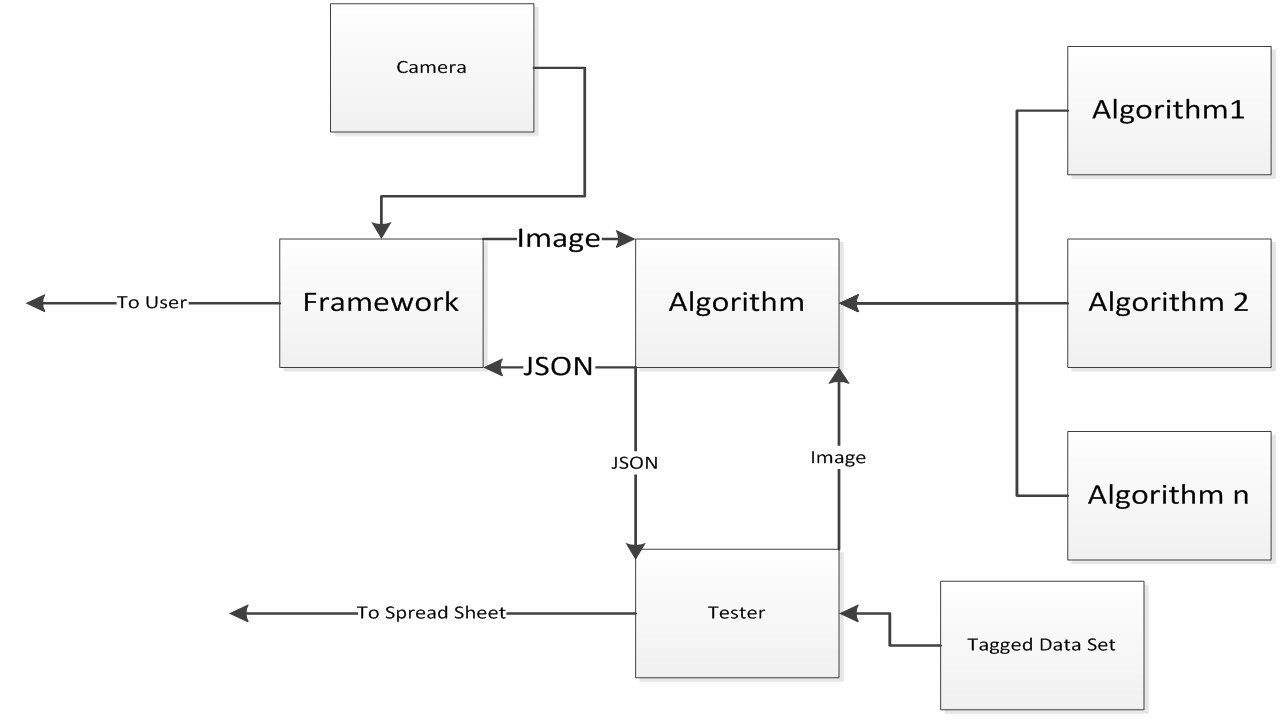
\includegraphics[width=0.8\textwidth,natwidth=610,natheight=642]{img/dataflow.jpg}
%    \caption{Basic workflow of stop sign detection.}
%\end{figure}

\subsection*{Development Framework}
\paragraph*{Usage}
The development framework, written in
framework\_images/framework\_cpp/framework.cpp from the root project directory,
is a C++ program that takes a command line argument, the path of the image to
process, and returns a 1 if the algorithm determined that the image contained a
stop sign or a 0 if not. An optional third argument can be provided to display
the image being classified. For example, to classify 
framework\_images/framework\_cpp/pos\_sample.jpg, an image containing a stop
sign, the proper usage is
\begin{lstlisting}
./framework pos_sample.jpg
\end{lstlisting}
to simply return the classification result without displaying it. To display
the image, this would be
\begin{lstlisting}
./framework pos_sample.jpg 1
\end{lstlisting}
although the actual value of the third argument does not matter, just its 
presence.
\paragraph*{Implementation Details}
The development framework includes the
framework\_images/framework\_cpp/algorithm.h header file that provides the 
interface the algorithms must be written to. This is the processImage function,
with the signature
\begin{lstlisting}
int processImage(Mat &img);
\end{lstlisting}
The framework loads the test image from the path specified in the command line 
argument onto memory with the OpenCV imread function as follows:
\begin{lstlisting}
Mat img = imread(argv[1], CV_LOAD_IMAGE_COLOR);
\end{lstlisting}
The second argument specifies the loaded image to be a 3 channel color image
and the output is stored in an OpenCV Mat object, a wrapper around a 
multi-channel 2-dimensional image array.

After loading the image, the image is processed and output is displayed. If
the render option is specified, 

\begin{lstlisting}
imshow(opencvtest, img);
\end{lstlisting}

displays the image being processed.
\subsection*{Algorithms}

\subsubsection*{Contour and Color Detection}
\paragraph*{Description and Usage}
Contour and color detection detects stop signs by finding the contours in the
image and searching the list of contours for the characteristic octagonal 
shape of the stop sign. A contour is a curve representing the boundary of a
region in the same color. Each contour is represented by an array of points.

If the octagonal contours were found, the algorithm returns immediately as 
there is a very high probability that the image contains a stop sign. If 
however, an octagonal contour was not found, the image is then processed for 
color detection to determine the percentage of red pixels. If the percentage is
higher than a specified threshold value, the image is classified as a stop 
sign.

This algorithm is linked to the framework and run by

\begin{lstlisting}
make alg_combine
./framework [path to image file]
\end{lstlisting}

\paragraph*{Implementation Details}
The implementation of Contour and Color Detection is provided in the file 
framework\_images/framework\_cpp/alg\_combine/alg\_combine.cpp from the root 
directory of our project. The RGB image is first converted to grayscale to make
edge detection simpler by removing the extra channels with 

\begin{lstlisting}
cvtColor(Img, Img_gray, CV_BGR2GRAY);
\end{lstlisting}

The Mat object Img\_gray now contains the grayscale image. A Gaussian Blur is
then applied to this grayscale image to smooth it and remove noise. 

\begin{lstlisting}
GaussianBlur(Img_gray, Img_gray, Size(3,3), 0);;
\end{lstlisting}

The resultant image is then passed through the Canny edge detector to detect 
the edges and threshold the image. 

\begin{lstlisting}
Canny(Img_gray, canny_output, thresh, thresh*2, 3);
\end{lstlisting}

These edges are then passed into the shapeDetect function, which searches for 
the 8-sided contour. The contours are first found by the OpenCV function 
findContours.

\begin{lstlisting}
findContours(img, contour, hierarchy, CV_RETR_LIST, CV_CHAIN_APPROX_SIMPLE, Point(0,0));
\end{lstlisting}

Then the algorithm loops through each contour found and approximates a 
polygonal curve from each.

\begin{lstlisting}
approxPolyDP(contour[i], result[i], epsilon, true);
\end{lstlisting}

If the curve is 8-sided and the area enclosed is greater than a specified
amount, the image is classified as stop sign. Otherwise, if no 8-sided contours
of the minimum area were found, the algorithm passes the original image through
color detection. This is done by first converting the original Mat object to
the HSV, or hue-saturation-value color space. This allows to focus simply on 
the hue component, or the color component and ignore differences in brightness,
accounted for by the saturation and value components. This is done by

\begin{lstlisting}
cvtColor(Img, imgHSV, COLOR_BGR2HSV);
\end{lstlisting}

The HSV image is then thresholded based on a specified hue threshold.

\begin{lstlisting}
Mat imgThresholded = colorDetect(imgHSV, Scalar(iLowH, iLowS, iLowV), Scalar(iHighH, iHighS, iHighV));
\end{lstlisting}

Finally, the percentage of red is found with the getFrac function and this is
compared with a minimum percentage of red and the image is classified as a 
stop sign or not stop sign. 
\subsubsection*{HOG}
The HOG algorithm works by extracting a HOG Descriptor from a 64x128 image window
this descriptor is then run through a SVM to see whether the window contains a 
stop sign. If it does the match is added to a vector of bounding rectangles which
represent the matches. The window is then shifted over a little bit and then rerun.
This repeats until the entire image has been processed. The matches are then run 
through non-maximum suppression to eliminate overlapping matches.

To run detector code you train a model to do this navigate to the hog directory. In
the git projects this is in $/framework\_images/framework\_cpp/hog/$. From there you can
run the command(assuming you have a tagged dataset):
\begin{lstlisting}
./trainer [path to dataset json] [path to output model] -c 200 -e 1e-6 -i 450 -o .5 -s 1.10 -r 5
\end{lstlisting}
The arguments:
\begin{itemize}
    \item c - C value for the SVM (See CVSVM documentation)
    \item e - Epsilon value for the SVM (See CVSVM documentation)
    \item i - Max number of iterations while training
    \item o - Amount of overlap required to be considered a true positive
    \item s - How much the image pyramid scales when trying to match (See gpu::HOG documentation)
    \item r - How many overlapping rectangles are required during suppression to be considered a match
\end{itemize}

This will take a while but once its done it will output some basic statistics 
on how the new training set performed. To use this trained model we have to copy it
to the models folder in the root git directory. With that done edit the name of the
module files used in $detector\_server.cpp$ on line 10 like so:
\begin{lstlisting}
svm.load(<absolute path model file>); 
\end{lstlisting}


The path must be absolute since we don't know what directory $0detector\_server$ will
be run in and we want to be sure it finds the model.

With that done we can now run it, to do that you will need two terminal sessions.
In the first run:
\begin{lstlisting}
make detector_server
./detector_server 
\end{lstlisting}

In the second navigate to to the $framework\_images/framework\_cpp$ directory and run:
\begin{lstlisting}
make hog_server
make test
\end{lstlisting}
The make test isn't necessary but it will test that the server is running properly.
Now you can use it like any other algorithm in the framework.

\subsubsection*{SURF and Bag of Words}
SURF and Bag of Words(BOW) are actually two algorithms that are used in conjunction to
classify an image. Classification is different than recognition in that it can't tell 
you where the stop sign is in the image, just that one exists. The algorithm works
in three stages:
\begin{enumerate}
    \item SURF is run over a tagged dataset, where it extracts the surf descriptors
        from any tags inside the image. These descriptors are added to a list.
    \item The list of all the descriptors is passed to a K-Means clustering algorithm
        that will find any groups of clustered points. These groups are then used to
        train a BOW vocabulary.
    \item We then run SURF over the full sized images in another test dataset. These
        SURF descriptors are then passed to BOW vocabulary which creates a new vector.
    \item This vector is then used to train a SVM. It is labeled positive if there is
        a tagged stop sign in the image, otherwise it is label a negative example. The
        SVM is then trained/
    \item To actually classify an image you just run 3 and 4 over an image but instead
        of training SVM you predict with it. If it predicts true there is a stop sign,
        otherwise there isn't.
\end{enumerate}

This algorithm ended up have some issues that should be kept in mind before using:
\begin{enumerate}
    \item It is slow, taking 1.5 seconds per a 400x300 image.
    \item It is only kind of accurate, the best was 72% accuracy.
    \item It is proprietary, meaning that you can't use it in any final commercial project.
        Additionally NVidia doesn't include it in the optimized OpenCV library
        which means that you will have to give up the OpenCV optimizations
        to use this algorithm on the jetson.
\end{enumerate}

To use this algorithm we first need to train it. To do this we will navigate to the
$/framework\_images/framework\_cpp/bow/$ in the git path. Once there we can run:
\begin{lstlisting}
make trainer
./trainer [taged dataset .json] [name of file to save the model to] [name of file to save vocab to]
\end{lstlisting}

You will notice that this outputs two files, the first is the SVM model, the second 
contains the vocabulary object. Both of these files should be copied to to models 
folder. Next edit detect.h and set the MODEL and VOCAB constants to be the absolute
path to the files that were just created. To run the detector you need to naviagte 
down to the $framework\_cpp$ directory. Build and run it using:
\begin{lstlisting}
make bow
make test
\end{lstlisting}

\subsubsection*{ROI}

\subsection*{Testing Framework}

The testing framework is pretty straight forward and requires two prerequisites:
\begin{enumerate}
    \item The main framework is already compiled with the algorithm you want to run
    \item You have a tagged dataset with the corresponding .json file 
\end{enumerate}
With that done to run the testing framework use:
\begin{lstlisting}
./tester [json file] [path to the result .csv you want create] [path to the framework executable]
\end{lstlisting}
This will create a .csv file with the result statistics for the algorithm.

\subsection*{Test Dataset}

\section*{Resources}
% What web sites were helpful (Listed in order of helpfulness)
% What, if any, reference books really helped?
% Were there any people on campus that were really helpful?
The following websites were particularly helpful:

\begin{enumerate}
    \item http://docs.opencv.org/
    We made heavy use of the OpenCV C++ documentation. It provided most of the
    functionality we needed to write our algorithms.
    \item http://stackoverflow.com/
    Stack Overflow was a great website to debug problems in our implementation
    as well as learn more about the internals of some of the OpenCV functions
    we leveraged.
    \item http://www.cse.iitd.ernet.in/~pkalra/csl783/canny.pdf
    This source provided useful information about the implementation of Canny
    Edge detection.
    \item http://opencv-srf.blogspot.com/2010/09/object-detection-using-color-seperation.html
    This is an OpenCV blog that had useful information about color detection
    and shape detection.
\end{enumerate}

In addition to these websites, we would like to give a big thank you to our 
mentors Matthew Zochert, Carl Price and Don Reid for their insights into 
stop sign recognition algorithms, hardware considerations and so much more. 

Last but not least, we would like to give a big thank you to our Senior Design
supervisor Professor Kevin McGrath and our TA throughout the year Jon Dodge for
making this project possible and for their support and insights into our 
project. 

\section*{What We Learned}
% What technical information did you learn?
% What non-technical information did you learn?
% What have you learned about project work?
% What have you learned about project management?
% What have you learned about working in teams?
% If you could do it all over, what would you do differently?
\subsection*{Hari Caushik}
By contributing to this project, I learned a fair bit of technical information. 
I improved my C++ programming skills and gained a familiarity with the OpenCV
library. In addition, I learned about the major concepts in computer vision
algorithms as well as image processing techniques. Throughout this project, I
also learned about software design practices and made practical use of
algorithmic complexity analysis.

A lot of non-technical information was also learned by doing this project. This
project required a lot of documentation at the start while we were 
determining the specifications, during the implementation when we documented 
the pseudocode and algorithmic complexity of the algorithms as well as our 
final report. My technical writing skills have improved as a result. We also 
presented our project, particularly towards the end of the year at the 
Engineering Expo to the general public, at ON Semiconductor to ON employees and
our final presentation video. 

Doing a nine month project for an actual client in industry has taught me most
of all that the main challenge is carefully defining an initially very 
loosely defined problem. Decisions that we make early on can have a very 
significant effect on the way our project may turn out. I have also learned 
that projects in the real world are very malleable. While the high level 
decisions we make early on guide our project in certain directions, specific 
requirements frequently change as we gain more knowledge through 
implementation. 

This project allowed each of use to take a project management role at different
times throughout the year. I learned most of all that establishing clear 
communication among all team members is essential to moving the project along 
smoothly. It is much easier to perform when each of us knows what is expected
of us and have clearly defined responsibilities. When this breaks down, there 
tends to be a lot of confusion and consequently inaction. 

I thoroughly enjoyed working with my team members and I feel as if things 
moved along very smoothly throughout the year. I learned how my teammates work
throughout the year and which ways I would need to adapt to make it work and
in which ways I could keep the same work habits. Overall I am very proud and 
impressed by my teammates' work and abilities and learned a lot technically
from them as well. Everyone compromised and contributed to the project. 

If I could do this project again, I would take a few more risks and attempt to
implement algorithms that were a little more advanced and would predict stop 
signs much more accurately. I wanted to ensure that we had moved the project 
forward this year. In hindsight, I think I was too conservative and wished I 
had been a little bolder.

\subsection*{Lane Breneman}

%What technical information did you learn?
Before this project I had used OpenCV for object recognition. That said I had
no experience working with the C++ interface and very little C++ experience in
general. Through this project I learned a lot about linking libraries, creating
make files and using classes in C++. On a different note I also learned a lot
about SVMs and machine learning. I had attempted to use these tools but had
never made much progress, but after this project I feel I have the skills to
employ them in future projects.

%What non-technical information did you learn?
I learned about taking notes and extracting the important information from 
research papers in order to reimplement their algorithms. I also learned 
how important communication between team members is. This largely came from
the fact the two of our basic algorithms turned out to be very similar and 
two of our advanced algorithms are also kind of similar. This limited the
variety of algorithms we explored, thus lowering the quality of the project.

%What have you learned about project work?
Our project integrated really nicely together, a large part of this I 
attribute to our good design. We found that we almost never needed to
fight the framework in order to get our code to run, which is nice. 
Even when last minute we need to make a way to export videos it took 
about 5 minutes to extend the framework. This reinforced the most 
import fact that I knew about project work, that a good design is 
important.

%What have you learned about project management?
Project management was a very mixed bag for our project. In the 
beginning we had very good project management, planning everything,
dividing work and communicating often. This lead to the best parts
of out project namely the framework and testing framework. Our later work
were less thought out and more divided and I feel that it can be seen in
quality of the work, as our algorithms could have been better.

%What have you learned about working in teams?
Communication is key. We had a really great group and I enjoyed working on the
project, but for most of the term the project became mostly individual. This lead
to two of our algorithms being pretty much the same. If we had communicated in 
more detail we could have seen this sooner and adapted.


%If you could do it all over, what would you do differently? 
If I could make one change I would have done 1 advanced algorithm each that we worked on over the year.
By advanced I mean more complicated than even the HOG or SURF algorithms. I feel
the project would of had more to show and been more rewarding if we had.

\subsection*{Joshua Deare}

\section*{Appendix 1: Essential Code Listings}

\section*{Appendix 2: Other Material}

\end{document}
